\documentclass{article}
\usepackage[utf8]{inputenc}
\usepackage{amsmath}
\usepackage{amssymb}
\usepackage{amsthm}

\usepackage{amsmath}
\usepackage{amssymb}
\usepackage{amsthm}
\usepackage{amscd}
\usepackage{amsfonts}
\usepackage{mathtools}

\usepackage[
backend=biber,
style=alphabetic,
sorting=ynt
]{biblatex}


\newtheorem{proposition}{Proposition}
\newtheorem{remark}{Remark}


\newcommand{\RR}[0]{\mathbb{R}}
\newcommand{\EE}[0]{\mathbb{E}}
\newcommand{\bx}[0]{{\bf x}}
\newcommand{\bv}[0]{{\bf v}}
\newcommand{\balpha}[0]{{ \bf\alpha}}
\newcommand{\HamiltonJacobiPDE}[2]{
%#1: Value function, #2: independent running cost
#1_t (x,t) + H(x,D_x #1(x,t)) = #2
}
\newcommand{\HamiltonJacobiTerminalCondition}[2]{
%#1: Value function, #2: Terminal payoff
#1(x,T) = #2(x)
}


\newcommand{\DensityTransportPDE}[2]{
    % #1: Value function, #2: Density
    #2_t(x,t) + \Delta(H_p(x, D_x #1 (x,t)) #2(x,t)) = 0
}

\newcommand{\DensityTransportInitialCondition}[1]{
    % #1: Density
    #1(x,t_0) = #1_0(x)
}


\newcommand{\ReducedMfgStateEvolution}[2]{
\begin{equation}\label{reduced_mfg:state_evolution}
\begin{cases}
    \dot{ #1}_t = {#2}_t,\quad t\in (t_0,T],\\
    {#1}_{t_0} = #1_0.
\end{cases}
\end{equation}
}

\newcommand{\ReducedMfgPayoffFunctional}[5]{
\begin{equation}\label{reduced_mfg:payoff_functional}
J({\bf #2},#1; t_0) = \int_{t_0}^T \left(#3({\bf #2}_s,{\bf #1}_s) + #5 \right) ds + #4({\bf #1}_T),
\end{equation}}

\newcommand{\ReducedMfgHamiltonian}[4]{
\begin{equation}\label{reduced_mfg:HJ}
H(#1,#2) \coloneqq \sup_{#3} ( #2 \cdot #3 + #4(#3,#1)).
\end{equation}
}


\newcommand{\ReducedMfgStateHamiltonJacobiTerminalValueProblem}[3]{
\begin{equation}\label{reduced_mfg:state_evolution_hamiltonian}
\begin{cases}
    \HamiltonJacobiPDE{#1}{#2}, \\
    \HamiltonJacobiTerminalCondition{#1}{#3}.
\end{cases}
\end{equation}}

\newcommand{\ReducedMfgFeedbackStateEvolution}[3]{
\begin{equation}\label{reduced_mfg:feedback_state_evolution}
\begin{cases}
    {\dot {\bf #1}}_#2 = H_p({\bf #1}, D_x #3({\bf #1},#2)),\\
    {\bf #1}_{t_0} = #1.
\end{cases}
\end{equation}}


\newcommand{\ReducedMfgDensityTransportInitialValueProblem}[2]{
\begin{equation}\label{reduced_mfg:density_transport_pde}
\begin{cases}
    \DensityTransportPDE{#1}{#2},\\
    \DensityTransportInitialCondition{#2}
\end{cases}
\end{equation}}

\newcommand{\ReducedMfgMeanFieldGameSystem}[4]{
\begin{equation}\label{reduced_mfg:mean_field_game_pde}
\begin{cases}
    \HamiltonJacobiPDE{#1}{#4},\\
    \DensityTransportPDE{#1}{#2},\\
\end{cases}
\end{equation}}

\newcommand{\ReducedMfgMeanFieldGameBoundaryConditions}[4]{
\begin{equation}\label{reduced_mfg:mean_field_game_boundary}
\begin{cases}
    \HamiltonJacobiTerminalCondition{#1}{#3},\\
    \DensityTransportInitialCondition{#2}.
\end{cases}
\end{equation}}



\addbibresource{sample.bib}

\title{Qualificação}
\author{Felipe Antunes}
\date{\today}

\begin{document}

\maketitle


\section{Introduction}

Mean field games is a branch of game theory, which is a set of concepts, mathematical tools, theorems, simulations methods and algorithms intended to model situations where agents make decisions strategically. Mean field game theory focus specifically a game with an infinite number of identical (symmetric) players. The infinite number of players are represented by their probability distribution over the state (or action) space.

Analysis of MFG focus on the interaction between a representative player sampled from the distribution, and the distribution itself. In essence, the representative player formulates his best response to the crowd. However, as every player is equal, the best response of the representative player determines the evolution of the crowd.


Applications focus mostly on Nash equilibria or social optimum, respectively mean field game and mean field control.
Mean field games concern the "competitive" setting, where each player decides his actions by means of solving  his own optimization problem. Mean field control, on the other hand, describe the "cooperative" setting, where the player's actions are derived from an optimization problem on the player's distribution as a whole. 

As an illustrative example, consider crowd motion: a crowd in a music festival could be modelled as a mean field game, with each individual attempting to optimize his position considering the loudness and the crowd's density. However, a military parade could be modelled as a mean field control, with each individual given orders to follow by a commander who wants to optimize the troop's distribution. 

In both cases, the optimality conditions give rise to coupled equations with a forward-backward structure: the forward equation describe the evolution of the distribution of players, while the backward equation describes the optimization problem for the representative player. The problem can be formulated in an analytical approach or in a probabilistic approach. 
In the analytical formulation, we have a system composed of a Fokker-Plank PDE with initial condition and a Hamilton-Jacobi-Bellman PDE with terminal condition \cite{lasry2007mean}.
As for the probabilistic formulation, we have a system of Forward-Backward SDE with McKean-Vlasov interactions \cite{carmona2013mean}. 

\if{
Some fields of application for MFG are 
\begin{itemize}
    \item economics: financial engineering [citations] and macroeconomic models [citations],
    \item population dynamics [citations], crowd motion [] and epidemiology [citations]
    \item engineering: energy production and management [citations], security and communication [citations], autonomous vehicles [citations].
\end{itemize}
}\fi

\subsection{An example from economics}
%%%%%%WIP%%%%%
We'll consider an example from economics in order to illustrate the mean field games methodology.
The model was chosen as an example for two reasons.
First, the mean field interactions arise naturally from the underlying economic theory, which makes the example a fitting introduction.
Second, the model is similar in nature to the educational model that we shall propose in sectio~\ref{sec:model_proposal}.

The example will be formulated in the deterministic setting, where the Nash equilibrium can be formulated using Pontryagin's Maximum Principle 
as the solution to a system of forward-backwards ODEs.

Consider an idealized economy composed of $N$ agents, with an optimization interval from time $t = 0$ to $t = T$.
Each agent has an amount of capital $k_0^i$ for $i \in \{1,\ldots,N\}$ at time $0$, and they're able to control their c~nsumption $c_t^i \in \RR$ over time.
The capital dynamics over time $\dot k_t^i$ is governed by two factors:
a fixed depreciation rate $\delta$ and an endogenous interest rate $r_t$. It is given by the ODE
\begin{equation}
    \dot k_t^i = \left[r_t - \delta \right] k_t^i - c_t^i. 
\end{equation}

Let's assume that the aggregate production $Y_t$ in the economy is given by a function $F$ of the aggregate capital of the economy $\hat k_t$, that is
\begin{equation}
    Y_t = F(\hat k_t),\quad \text{where } \hat k_t = \frac{1}{N} \sum_{i = 1}^N k_t^i.
\end{equation}
In economic equilibrium, the interest rate $r_t$ will be determined by the marginal effect of capital $\partial_K Y$ in the aggregate production,
which itself is a function of the aggregate capital in the economy $K_t$. This will be the source of mean field interactions for our model.

The preference for consumption of the agents is given by an utility function $u(c_t^i)$, 
and their preference for capital at the end of their lifetime is given by a terminal cost $\psi(k_T^i)$.
Therefore, agents want to choose their consumption $c(\cdot)$ to optimize the following functional $J(k, c(\cdot))$:
\begin{equation}
    J(k, c(\cdot)) = \int_0^T u(c(s)) ds + \psi(k_T),
\end{equation}
where $k$ is the starting capital, and $k_T$ is the capital at time $T$ when following control $c(\cdot)$.
Therefore, the optimization problem faced by agent $i$ is
\begin{equation}\label{economic_example:N_player_game}
    \begin{cases}
        \max_{c^i_{(\cdot)}} \int_0^T u(c^i_s) ds + \psi(k^i_T),\\
        \text{subject to}\\
        \dot k_t^i = \left[ \partial_K F(\hat k_t) - \delta \right] k_t^i - c_t^i.
    \end{cases}
\end{equation}

In the mean field game framework, instead of directly solving the $N$-player model~\eqref{economic_example:N_player_game},
we solve a different but related problem. 
We modify the setting of the game from $N$ players distributed at time $t$ according to a discrete probability measure $\mu^N_t$ to infinite players
distributed according to an atomless probability distribution  $\mu_t$.
This new setting is the mean field game, and under appropriate conditions its Nash equilibrium is an approximate Nash equilibrium for the $N$ player game.

We're now in position to analyze the model. Analysis of mean field games models have the following pattern:
\begin{enumerate}
    \item Find the optimal control for a representative player, given a flow of probability measures $\mu_t$,
    \item As every player is equal, their optimal trajectories induce a flow $O(\mu_t)$,
    \item A Nash equilibrium for the MFG is a probability flow $\mu_t^*$ such that $\mu_t^* = O(\mu_t^*)$.
\end{enumerate}
By definition, a Nash equilibrium is a state of the game where no player can improve his outcome by unilaterally changing his strategy.
The measure flow $\mu_t^*$ induces its own time evolution when every player behaves optimally.
This means they can't improve their outcomes any more,
which means that the mean field definition of Nash equilibrium is compatible with the classical definition.
 
Let's set $u(c) = \log(c)$ and $\psi(k) = - \frac{1}{2} k^2$.
Moreover, let's denote $\hat k_t = \int k_t d \mu_t$ and set $F(K) = \frac{C}{2} K^2$, that is, there are increasing returns over aggregated capital.
In this setting, the interest rate is given by $r_t = C {\hat k_t} $.
Assuming that an initial capital $k \sim \mu_0$ is given,
the representative agent faces the following optimization problem:
\begin{equation}\label{economic_example:representative_agent}
    \begin{cases}
        \max_{c_{(\cdot)}} \int_0^T \log(c_s) ds -\frac{1}{2}{(k_T)}^2,\\
        \text{subject to}\\
        \dot k_t = \left[ C {\hat k_t} - \delta \right] k_t - c_t, \quad k_0 = k,
    \end{cases}
\end{equation}

Assuming that ${\hat k_t}$ is given, we can apply Pontryagin's Maximum Principle~\ref{ADD STATEMENT TO APPENDIX AND CITATION}
to conclude that, if an optimal control $c^*_{(\cdot)}$ and a corresponding optimal trajectory $k^*_{(\cdot)}$ exist,
then there is a costate variable $p_{(\cdot)}$ defined implicitly as the solution of the backwards ordinary differential equation
\begin{equation}\label{economic_example:costate_ode}
    \dot p_t = -  \left[C{\hat k_t} - \delta \right] p_t, \quad p_T =  - k^*_T,
\end{equation}
that satisfy the maximality condition
\begin{equation}\label{economic_example:maximality_condition}
    p_t\left( \left[C {\hat k_t} - \delta \right]k^*_t - c^*_t \right) + \log(c^*_t) = 
    \max_c \left\{ p_t\left( \left[C {\hat k_t} - \delta \right]k^*_t - c \right) + \log(c) \right\}.
\end{equation}

We can find candidates for optimal controls and trajectories by calculating
\begin{equation*}
    c^* = \arg\max_c  \left\{ p_t\left( \left[C {\hat k_t} - \delta \right]k^*_t - c \right) + \log(c) \right\} = \frac{1}{p_t},
\end{equation*}
and solving the forward-backward system of ordinary differential equations
\begin{equation}\label{economic_example:ode_formulation}
    \begin{cases}
         \dot k_t = \left[ C {\hat k_t} - \delta \right] k_t - \frac{1}{p_t},\\
         \dot p_t = -  \left[C{\hat k_t} - \delta \right] p_t, \\
         k_0 = k,\, p_T =  - k_T.         
    \end{cases}
\end{equation}
\begin{remark}
    Note that $k_t$ is actually a random variable dependent on its initial value $k\sim \mu_0$.
    The system of ODEs implicitly describes the probability measure flow $\mu_t = \mathcal{L}(k_t)$,
    and the dynamics of this forward-backward system depend on $\mathcal{L}(k_t)$ through $\hat k_t$.
    In the stochastic case, the dependence on the law is the distinguishing feature of McKean-Vlasov SDEs.
\end{remark}
    Pontryagin's Maximum Principle give us \textit{necessary} conditions for optimal controls and trajectories, but not \textit{sufficient} conditions.
    In order to guarantee optimality, one method is to analyze the value function $V$ defined as
\begin{equation}\label{economic_example:value_function_definition}
    V(k,t) = \sup_{c_{(\cdot)},\, k_t = k} \int_t^T \log(c(s)) ds -\frac{1}{2}{(k_T)}^2.
\end{equation}
Intuitively, the value function evaluates for a given time $t$ and capital $k$ the optimal payoff from that point forward.
As shown in section~\ref{ADD_APPENDIX_FOR_VISCOSITY_SOLUTIONS}, the value function is the viscosity solution for the Hamilton-Jacobi-Bellman equation
\begin{equation}\label{economic_example:hjb_equation_reduced}
    \begin{split}
        &\partial_t V + H(\partial_k V, k,t) = 0,\quad V(k,T) = -\frac{1}{2}{(k)}^2,\\
        &\text{where }
        H(p,k,t) = \sup_{c} p\left[ \left(C {\hat k_t - \delta}\right)k - c \right] + \log(c).
    \end{split}
\end{equation}
This equation encodes the system of ODEs in~\ref{economic_example:ode_formulation} through the Hamiltonian function by the relations
\begin{equation*}
    \dot k_t = \partial_p H,\, \dot p_t = -\partial_k H.
\end{equation*}
Moreover, as shown in~\ref{ADD_APPENDIX_FOR_TRANSPORT_EQUATION_AND_FKP},
when the agents' capital evolve according to $\dot k = \partial_p H$,
the probability density function $\rho(\cdot, t)$ for the agents probability measure $\mu_t$ at time $t$
is the weak solution for the Kolmogorov-Fokker-Planck equation with initial condition $\rho_0$ given by the pdf of $\mu_0$
\begin{equation}\label{economic_example:fkp_equation_reduced}
\begin{split}
    &\partial_t \rho - \partial_k \left( \partial_p H \rho \right) = 0, \rho(k,0) = \rho_0.
\end{split}
\end{equation}
In the Nash Equilibrium, the capital per capita at time $t$ is a function of $\rho$ given by $\hat k_t(\rho) = \int_{\RR} k \rho(k,t) dk$.
Substituting 
\begin{equation*}
    H(p,k,t) = \left(C {\hat k_t(\rho) - \delta}\right)k p  - 1  - \log(p)
\end{equation*}
on~\ref{economic_example:hjb_equation_reduced} and~\ref{economic_example:fkp_equation_reduced}, we have the full PDE system
\begin{equation}
    \begin{cases}
        \partial_t V +  \left(C {\hat k_t(\rho) - \delta}\right)k\partial_k V - 1  - \log(\partial_k V) = 0,\quad V(k,T) = -\frac{1}{2}{(k)}^2,\\
        \partial_t \rho - \partial_k \left( \left[ \left(C {\hat k_t}(\rho) - \delta\right) k - {(\partial_k V)}^{-1} \right]\rho \right) = 0, \rho(k,0) = \rho_0.
    \end{cases}
\end{equation}
\color{black}




\section{Theoretical Review - Mean Field Games Theory}

\subsection{Theoretical Review outline}

Mean field games are a framework for approximating Nash equilibria of certain kinds of games with a large number of players.
There are two equivalent ways of formulating a mean field game - through a system of coupled partial differential equations, or through a system of forward-backward stochastic differential equations.

In this section, we will explore the theory of mean field games.
We will begin by reviewing important concepts in game theory. 
Then, we shall review both the PDE system point of view and the FBSDE point of view. 
Equiped with an understanding of both point of views, we will analyze the limit of N-player games and its relationship to MFG.
Following the theoretical subsections, we will explore numerical solutions for MFG and applications.
We shall end the section by analyzing a model for human capital development.
We refer the reader to Appendix \ref{appendix-game-theory} for a review of game theory concepts, and to Appendix \ref{appendix-mathematical-background} for a review of necessary mathematical background.


\subsection{Three roads for Mean Field Games Theory}

Conceptually, there are three approaches to mean field games theory - from physics, from game theory and from economic theory.

\subsubsection{First road: from physics to mean field games}

% To do
% Add an physical example - i.e. gravity vs termal pressure model
In particle physics, situations with large number of particles are handled using mean field theory. Instead of modelling all the inter-particle interactions, one introduces a "mean field" which serve as mediator for the interactions. Each particle both contributes to and is influenced by the mean field.

In order to use this approximation, the inter-particle interactions must be sufficiently weak or regular.

Mean field game theory adapts this methodology to situations in which agents interact in strategic situations. The challenge is to take into account not only the ability of agents to make decisions, but also the interaction between strategies: each player's strategy tries to take into account the other player's strategy.
\textbf{This changes the nature of the mean field: it is not an statistic on the domain of particle states anymore, but rather a statistic on the domain of strategies and information.}

Although the term "mean-field" is borrowed from Physics, mean field game theory does not restrain itself to applying physical models to economy. Instead, as a branch of game theory, mean field games models aim to \textit{explain} rational behaviour through the structure of the agent's interactions and payoffs. \cite{cousin2010paris}

\subsubsection{Second Road: From Game Theory to Mean Field Games}

In game theory, $N$-player games quickly become intractable as $N$ gets large. Mean Field Games provide a way to approximate the limiting case as $N \to \infty$ for a class of $N$-player game which respect a form of anonymity: direct interactions between players are comparatively small, and players can be interchanged without changing the interaction. This is the case when interactions are mediated through some average of the player's state, for instance.
The mean field approach consists in approximating the $N$ players by a continuum of players distributed through the state space. Each agent formulates his optimal response given the distribution of players, and conversely this optimal response implies an evolution through time for the player's distribution.
\textit{In layman's terms, each player formulates his strategy against the crowd, and the crowd evolves according to each player's strategy.}

\subsubsection{Third Road: From Economics to Mean Field Games}
% To Do
% Add toy model with general equilibrium, reference it here
In economic models following the Theory of General Economic Equilibrium, interactions are mediated by prices. Direct interactions of agents are excluded from these economic models. However, systemic economic effects such as externalities, public goods, etc give rise to interactions which are not mediated by price. Both price formation and systemic effects can be modelled by a mean field type model. This way, MFG theory lends itself as a tool of economic analysis.



\subsection{Analytical point of view}
%% To do
% - Write as system of forward backward ode's
% - write as system of PDE's
\usepackage{amsmath}
\usepackage{amssymb}
\usepackage{amsthm}
\usepackage{amscd}
\usepackage{amsfonts}
\usepackage{mathtools}

\usepackage[
backend=biber,
style=alphabetic,
sorting=ynt
]{biblatex}


\newtheorem{proposition}{Proposition}
\newtheorem{remark}{Remark}


\newcommand{\RR}[0]{\mathbb{R}}
\newcommand{\EE}[0]{\mathbb{E}}
\newcommand{\bx}[0]{{\bf x}}
\newcommand{\bv}[0]{{\bf v}}
\newcommand{\balpha}[0]{{ \bf\alpha}}
\newcommand{\HamiltonJacobiPDE}[2]{
%#1: Value function, #2: independent running cost
#1_t (x,t) + H(x,D_x #1(x,t)) = #2
}
\newcommand{\HamiltonJacobiTerminalCondition}[2]{
%#1: Value function, #2: Terminal payoff
#1(x,T) = #2(x)
}


\newcommand{\DensityTransportPDE}[2]{
    % #1: Value function, #2: Density
    #2_t(x,t) + \Delta(H_p(x, D_x #1 (x,t)) #2(x,t)) = 0
}

\newcommand{\DensityTransportInitialCondition}[1]{
    % #1: Density
    #1(x,t_0) = #1_0(x)
}


\newcommand{\ReducedMfgStateEvolution}[2]{
\begin{equation}\label{reduced_mfg:state_evolution}
\begin{cases}
    \dot{ #1}_t = {#2}_t,\quad t\in (t_0,T],\\
    {#1}_{t_0} = #1_0.
\end{cases}
\end{equation}
}

\newcommand{\ReducedMfgPayoffFunctional}[5]{
\begin{equation}\label{reduced_mfg:payoff_functional}
J({\bf #2},#1; t_0) = \int_{t_0}^T \left(#3({\bf #2}_s,{\bf #1}_s) + #5 \right) ds + #4({\bf #1}_T),
\end{equation}}

\newcommand{\ReducedMfgHamiltonian}[4]{
\begin{equation}\label{reduced_mfg:HJ}
H(#1,#2) \coloneqq \sup_{#3} ( #2 \cdot #3 + #4(#3,#1)).
\end{equation}
}


\newcommand{\ReducedMfgStateHamiltonJacobiTerminalValueProblem}[3]{
\begin{equation}\label{reduced_mfg:state_evolution_hamiltonian}
\begin{cases}
    \HamiltonJacobiPDE{#1}{#2}, \\
    \HamiltonJacobiTerminalCondition{#1}{#3}.
\end{cases}
\end{equation}}

\newcommand{\ReducedMfgFeedbackStateEvolution}[3]{
\begin{equation}\label{reduced_mfg:feedback_state_evolution}
\begin{cases}
    {\dot {\bf #1}}_#2 = H_p({\bf #1}, D_x #3({\bf #1},#2)),\\
    {\bf #1}_{t_0} = #1.
\end{cases}
\end{equation}}


\newcommand{\ReducedMfgDensityTransportInitialValueProblem}[2]{
\begin{equation}\label{reduced_mfg:density_transport_pde}
\begin{cases}
    \DensityTransportPDE{#1}{#2},\\
    \DensityTransportInitialCondition{#2}
\end{cases}
\end{equation}}

\newcommand{\ReducedMfgMeanFieldGameSystem}[4]{
\begin{equation}\label{reduced_mfg:mean_field_game_pde}
\begin{cases}
    \HamiltonJacobiPDE{#1}{#4},\\
    \DensityTransportPDE{#1}{#2},\\
\end{cases}
\end{equation}}

\newcommand{\ReducedMfgMeanFieldGameBoundaryConditions}[4]{
\begin{equation}\label{reduced_mfg:mean_field_game_boundary}
\begin{cases}
    \HamiltonJacobiTerminalCondition{#1}{#3},\\
    \DensityTransportInitialCondition{#2}.
\end{cases}
\end{equation}}



\addbibresource{sample.bib}
To Do
\begin{itemize}
    \item Cardaliaguet, Diogo Gomes
    \item System statement - HJB and FKP
    \item Existence of solutions - Viscosity Solutions
    \item Uniqueness
    \item Approximate Nash Equilibrium
\end{itemize}

\subsubsection{Reduced Mean-field games}\label{reduced_mfg}
Among the main motivations for studying MFG are the connections with
 the theory of $N$-player differential games. A solution of the MFG formalizes 
 the limit case of Nash equilibrium when $N \to \infty$ for $N$-person differential games.

Some reduced mean-field games models can be rigorously derived as the limit 
of equations characterizing an $N$-player differential game. This subsection presents a heuristic derivation.

Consider first the single-agent optimal control problem.
Suppose that the state of an agent at time $t$ is characterized by the vector 
$\state_t \in \RR^d$.
In addition, assume that the following differential equation describes the state $\state_t$:
\begin{equation}\label{reduced_mfg:state_evolution}
\begin{cases}
    \dot{ \state}_t = {\control}_t,\quad t\in (t_0,T],\\
    {\state}_{t_0} = \state_0.
\end{cases}
\end{equation}

where $\control_t$ is a control and $\state_0\in\RR^d$ is a given initial condition. This agent seeks to maximize the functional:

\begin{equation}\label{reduced_mfg:payoff_functional}
    J({ \control},\state; t_0) = \int_{t_0}^T \left(\cost({\control}_s,{\state}_s) + g[\rho] \right) ds + \cost_T({ \state}_T),
\end{equation}
where $\cost$ is a Lagrangian, $\cost_T$ is a terminal payoff and $g[\rho]$ is a term to be made precise later. 

Define the Hamiltonian
\begin{equation}\label{reduced_mfg:hamiltonian}
        H(\state,p) \coloneqq \sup_{\control} ( p \cdot \control + \cost(\control,\state)).
\end{equation}
We know from Section
\eqref{deterministic_optimal_control}
that under some regularity assumptions,the value function $V$ associated with
the optimal control problem
\eqref{deterministic_optimal_control:optimal_control_problem} 
solves the Hamilton-Jacobi equation in $\RR^d \times [t_0,T)$:
\begin{equation}\label{reduced_mfg:state_evolution_hamiltonian}
\begin{cases}
    \partial_t V (\state,t) + H(\state,\partial_x V(\state,t)) = g[\rho], \\
    V(\state,T) = \cost_T(\state).
\end{cases}
\end{equation}
Moreover, the optimal control $\control^*$ is given in feedback form by
$$\control^*(\state,t) = \partial_p H(\state, D_x V(\state, t)).$$
The state of a rational agent will evolve according to 
\eqref{reduced_mfg:state_evolution} with the control $\control$ equal to the feedback optimal control $\control^*$.

Consider then a continuum of rational and indistinguishable agents.
The distribution of agents is given by an atomless probability measure $\rho$.
This population of agents is subjected to the same optimal control problem.
Therefore, the state of each individual is driven by
\begin{equation}\label{reduced_mfg:feedback_state_evolution}
\begin{cases}
        {\dot {\state}}_s = \control^*(\state,t),\\
        {\state}_{t_0} = \state_0.
\end{cases}
\end{equation}
The function $g$ encodes the dependence of the agent's cost functional on the density of the entire population.
This implies that the optimization problem faced by the agents depends on the evolution of $\rho$.
Conversely, the evolution of $\rho$ depends on a vector field determined by $V$, which is derived from the control problem of the agents.
\footnote{Chicken and the egg problem.}

From Section
\eqref{transport_eq},
we know that if $\state$ satisfies
\eqref{reduced_mfg:feedback_state_evolution},
then the evolution of the density $\rho$ in time satisfies a transport equation in $\RR^d \times (t_0, T]$:
\begin{equation}\label{reduced_mfg:density_transport_pde}
    \begin{cases}
        \partial_t \rho(\state,t) + \nabla(\control^*(\state,t) \rho(\state,t)) = 0
        \rho(\state,t_0) = \rho_0(\state)
\end{cases}
\end{equation}
The mean-field game system associated with this problem is then the system of PDE's:

\begin{equation}\label{reduced_mfg:mfg_system}
    \begin{cases}
        \partial_t V (\state,t) + H(\state,\partial_x V(\state,t)) = g[\rho], \\
        \partial_t \rho(\state,t) + \nabla(\partial_p H(\state, \partial_x V (\state,t)) \rho(\state,t)) = 0
\end{cases}
\end{equation}
coupled with the boundary conditions

\begin{equation}\label{reduced_mfg:mfg_boundary_conditions}
\begin{cases}
    V(\state,T) = \cost_T(x), \\
    \rho(\state,t_0) = \rho_0(\state)
\end{cases}
\end{equation}




\subsection{Probabilistic point of view}
%% To do
% Write as system of second order pde's
\begin{itemize}
    \item Reference - Carmona's Book.
    \item Intro and Definitions - 3.2
Mean Field Games can be proposed as a system of Forward-Backward Stochastic Differential Equations (FBSDEs). In order to illustrate this, we will construct the system, following the same logical development as in Section \ref{PDE_formulation_section}

Suppose a typical player formulates his best response given the actions of all other players. This amounts to solving an optimal control problem
\begin{equation}
\begin{split}
\begin{cases}
   \inf_{\alpha \in \mathbb{A}} \EE \left[ \int_0^T f(t,X_t, \mu_t, \alpha_t) dt + g(X_T, \mu_T)\right]  \\
    \text{subject to}\\
     dX_t = b(t,X_t, \mu_t, \alpha_t) dt + \sigma(t, X_t, \mu_t) dW_t, \\ 
     t \in [0,T], X_0 = \xi.
\end{cases}
\end{split}
\end{equation}
    Where $X_t$ is the state of the typical player, $\alpha_t$ is the player's action, and $\mu_t$ represents the impact of the strategies chosen by other players. We assume there is no control in $\sigma$. In the case of mean field games without common noise, $\mu_t$ is deterministic - it is the marginal distribution at time $t$ of the state of a generic player in the population.

    The value function for this optimal control problem has a probabilistic representation as the solution of a BSDE:
\begin{equation}
    \begin{split}
    \begin{cases}
        dY_t = - f(t,X_t, \mu_t, \alpha_t) dt + Z_t \cdot dW_t, \quad t \in [0,T],\\
        Y_T = g(X_T, \mu_T)
    \end{cases}
    \end{split}
\end{equation}
    where $(X_t)_{0 \leq t \leq T}$ is the controlled process obtained by choosing for $(\alpha_t)_{0\leq t \leq T}$ the specific control 
    $$
    \alpha_t = {\hat \alpha} \left( t, X_t, \mu_t, \left(\sigma(t,X_t,\mu_t)^{-1}\right)^{\dagger} Z_t \right), \quad t \in [0,T].
    $$
    
    If we require that the representative player behaves optimally, then $\hat \alpha$ is given by:
    $$
    {\hat \alpha} \left( t, x, \mu, y \right) \in \arg\min_{\alpha \in A} H(t,x,\mu,y,\alpha),
    $$
where $H$ is the reduced Hamiltonian 
$$H(t,x,\mu,y,\alpha) = y\cdot b(t,x,\mu, \alpha) + f(t,x,\mu, \alpha).$$
This choice for $\alpha_t$ couples $dX_t$ and $dY_t$ into a BSDE with deterministic coefficients taking the measure flow $(\mu_t)_{0 \leq t \leq T}$ as input.
Setting 
$$
B(t,x,\mu,y,z) = b\left(t,x,\mu, {\hat \alpha} (t,x,\mu,\sigma(t,x,\mu)^{-1 \dagger}  ))\right),
$$
$$
F(t,x,\mu,y,z) = f\left(t,x,\mu, {\hat \alpha} (t,x,\mu,\sigma(t,x,\mu)^{-1 \dagger}  ))\right)
$$
we have the following FBSDE:
\begin{equation}
\begin{split}
     \begin{cases}
         dX_t = B(t,X_t,\mu_t,Y_t,Z_t) dt + \sigma(t,X_t,\mu_t) dW_t,\\
         dY_t = - F(t,X_t,\mu_t,Y_t,Z_t) dt + Z_t dW_t, \quad t \in [0,T],\\
         Y_T = G(X_T, \mu_T).
     \end{cases}   
\end{split}
\end{equation}

Finally, note that in the Nash equilibrium every agent is behaving optimally. This means that the flow of the population distribution represented by 
${\bf \mu} = (\mu_t)_{0 \leq t \leq T}$  
should match the flow of marginal distributions of states for the representative agent - that is, the law
$\mathcal{L}(X_t)_{0 \leq t \leq T}$
of the forward process 
$(X_t)_{0 \leq t \leq T}$.

Writing the resulting McKean-Vlasov FBSDE in full:
\begin{equation}
\begin{split}
     \begin{cases}
         dX_t = B(t,X_t,\mathcal{L}(X_t),Y_t,Z_t) dt + \sigma(t,X_t,\mathcal{L}(X_t)) dW_t,\\
         dY_t = - F(t,X_t,\mathcal{L}(X_t),Y_t,Z_t) dt + Z_t dW_t, \quad t \in [0,T],\\
         Y_T = G(X_T, \mathcal{L}(X_T)).
     \end{cases}   
\end{split}
\end{equation}

\item Commentario no paralelo entre formulação estocástica e formulação analítica
\item Existência - SMP, Unicidade - Lasry Lions Monoticity

    \item FBSDE - 3.2
    \item LQ MFG 3.5
\end{itemize}


\subsection{N-player game limit point of view}
To Do
\begin{itemize}
    \item What is the limit of a game with respect to the number of players? What notion of limit are we considering?
    \item Under what conditions can we guarantee that the mean field game approximates the N-player game?
    \item Follow Cardaliaguet's approach
\end{itemize}



\subsection{Numerical Solutions - Classical}


Most methods are based on optimality conditions in terms of PDEs or SDEs with suitable discretization schemes, such as finite differences, semi-Lagrangian schemes or probabilistic approaches. These methods are well understood and work well in small dimensions. However, these methods do not perform so well for MFG with high dimensional states or controls, as they suffer from the curse of dimensionality.
To Do
\begin{itemize}
    \item Refer to Lauriere notes on numerical solutions
\end{itemize}

\subsection{Numerical Solutions - ML}
Stochastic methods based on Neural Networks have been proposed as a solution for the dimensionality limitation of classical methods.
To Do
\begin{itemize}
    \item Refer to Lauriere Learning MFG
    \item Artigo Yuri
\end{itemize}

\subsection{Applications}
To Do
\begin{itemize}
    \item Follow Carmona's application review
    \item Carmona's article 
    
    Applications in Financial Engineering:Systemic Risk, Price Impact and optimal execution, Models for Bank runs
    
    Applications in Energy Markets and Environment: MFG Models for Oil Production, MFG models for the eletricity markets and the Grid, Environment Economics.

    Applications to Macroeconomic Growth Models

    Applications to Contract theory and moral hazard.
\end{itemize}


\section{Model Proposal}
We propose a game theoretical model for time allocation between work and education.
The model is based on Lucas's human capital growth model \cite{lucas1988mechanics} and Aiyagari’s growth model \cite{achdou2014partial,carmona2018probabilistic}.
\textcolor{red}{Add paragraph about lucas model and paragraph about aiyagari's model.}
The agents interactions are mediated through the interest rate and wage rate of the economy, which depend on aggregated quantities of the agent's states.

\textcolor{red}{Elaborate on the justification for the interest rate and the wage rate.
Explain skill level/wage rate}

Some expected results of this research are qualitative properties and numerical solutions of the mean field limit of the game. \textcolor{red}{develop goals}

\subsection{Economic Theory Review}

\subsubsection{ Mean Field Models (or similar) in Economic Research}
\begin{itemize}
    \item Moll, Lucas
    \item Models for Heterogeneous Agents
    \item Gabaix, Dynamics of Inequality, 2016 - Sharp rise in inequality not modelled accurately by standard random growth models. The paper suggests some changes to standard models that address this issue: type dependence and scale dependence in wealth accumulation.
    \item TAPPING INTO TALENT - Model for economy where agents can chose between working on industry or working as a researcher. Has an educational component - agents can only chose to become researchers if they pursue an PhD. Pursuing a PhD has "innate talent" and economic restrictions. Researcher's wage are calculated by solving for the market equilibrium in a free market of ideas. Model is calibrated to census data from Denmark and used to study counterfactual policy exercises.
    \item Non market interactions - Scheinkman - check for more recent references
\end{itemize}

\subsubsection{Econometric Research on Education}
\begin{itemize}
    \item Articles with stylized facts - Tapping Into Talent
    \item articles that measure interesting behaviour that we hope the model can replicate.
    \item articles that argue in favor of the importance of this research
    \item Growth models review - specially Lucas and Ayiagari
\end{itemize}


\subsection{Model}
\begin{enumerate}
    \item Analysis
    \item Semi-analytic solution
    \item Comparison with N-player
\end{enumerate}

Consider an economy with $N$ agents, evolving in the time interval $[0,T]$.
Each agent is described at time $t$ by his wealth $A_t$ and his skill level $H_t$,
with $(A_t, H_t) \in \Omega = \mathbb{R} \times \mathbb{R}^+$ for every $t \in [0,T]$.
Agents control their consumption $c_t \in \mathbb{R}^+$, and the proportion of time they dedicate to working $u_t \in [0,1]$. 
We assume that the proportion $1 - u_t$ of time not used to working is used to improve their skill level. 

Each agent face the following optimization problem:
\begin{equation}
\begin{cases}
        \sup\limits_{(u,c) \in \mathcal{U} \times \mathcal{C}}\mathbb{E} [ \int_0^T f_c(c_s) + f_u(u_s) ds + Q(A_T) ], \text{ s.t.}\\
        d H_t = H^\xi_t g(1 - u_t) dt + \sigma_h H_t d W^h_t,\\
        d A_t = \left[ (\bar r_t - \delta) A_t + \bar w_t H_t u_t - c_t  \right] dt + \sigma_a A_t d W^a_t.
\end{cases}
\end{equation}
The term $f_c(c_s)$ is a running utility for consumption, whereas $f_u(u_s)$ is a running utility for proportion of time spent working.
The term $Q(A_T)$ represents utility over terminal wealth.

The agent's skill level $H_t$ evolves through time with a drift term $H^\xi_t g(1 - u_t) dt$ and a noise term $\sigma_h H_t dW^h_t$.
The function $g$ represents the effectiveness of time $1 - u_t$ employed in improving skill level,
 whereas the term $H_t^\xi$ captures the impact of current skill level in effectiveness of effort.
 For $\xi > 0$, higher skill levels lead to higher effectiveness.
  However, for $\xi < 0$, higher skill levels lead to lower effectiveness.
  As for $\xi = 0$, the skill level is indifferent to effectiveness.

The agent's wealth $A_t$ evolves with a drift term $\left[ (\bar r_t - \delta) A_t + \bar w_t H_t u_t - c_t  \right] dt $ and a noise term $\sigma_a A_t d W^a_t$.
The drift term is composed of interest returns over current wealth, wages proportional to time dedicated to working and a reduction on wealth due to consumption given by $c_t$.
The interest returns are described by $(\bar r_t - \delta) A_t$, where $\delta$ is a depreciation rate and $\bar r_t$ is the interest rate of the economy, to be determined endogenously through mean field interactions.
The wages are given by $\bar w_t H_t u_t$, where $H_t$ is the agent's skill level, $u_t$ is the proportion of time dedicated to work and $\bar w_t$ is the wage rate per time per skill of the economy, which also will be determined endogenously through mean field interactions.

The noise terms $\sigma_h H_t dW^h_t$ and $\sigma_a A_t dW^a_t$ are driven by independent brownian motions $W^h_t$ and $W^a_t$.
We consider that each agent has independent noise.

\textcolor{red}{elaborate on the aggregate quantities description}

Moreover, suppose that the production function $F$ for the economy depends on aggregate capital $\bar a$ and the effective supply of ability 
$\bar h^e$, and is given by a Cobb-Douglas function \cite{Add Refernce for Cobb-Douglas} as 
$$F(\bar a,\bar h^e) = k ({\bar a})^\beta ({\bar h^e})^{1-\beta}.$$

Suppose agents are distributed over $\Omega$ at time $t$ with a measure $\mu_t \in \mathcal{P}(\Omega)$.

Given an measure flow $(\mu_t)_{t \in [0,T]}$ and a feedback form for the control $u: u(a,h), $, we can calculate the aggregate quantities
\begin{equation*}
    \begin{cases}
        \bar a_t = \int_\Omega a\, d\mu_t(a,h),\\
        \bar h^e_t = \int_\Omega u(a,h)\, h d\mu_t (a,h).
    \end{cases}
\end{equation*}
The value $\bar a_t$ is the average wealth of the economy, whereas $\bar h^e_t$ is the effective supply of skilled labor in the economy - note that the the integral term is a weighted average of the skill $h$ level over the population distribution $\mu_t$, where the weights $u(a,h)$ are the proportion of time an agent with wealth $a$ and skill level $h$ devotes to work.

At economic equilibrium, the interest rate and wage per time per ability satisfy
$$\bar r_t = \partial_a F(\bar a_t, \bar h^e_t),\quad \bar w_t = \partial_h F(\bar a_t, \bar h^e_t).$$
\textcolor{red}{analyze monotonicity and convexity wrt. aggregate quantities}


Solutions for \eqref{education_model:mfg_analytic_system} describe Nash equilibria for the mean-field limit of the game.
The function $V: [0,T] \times \Omega \mapsto \mathbb{R}$ is the value function for the game at the Nash equilibrium,
whereas the probability measure flow $\mu: [0,T] \times \Omega \mapsto \mathbb{R}$ describe the time evolution of the  population density over the state space $\Omega$.
\begin{equation}\label{education_model:mfg_analytic_system}
    \begin{cases}
        \partial_t V + (\bar r  - \delta) a \partial_a V + \HH_u  + \HH_c + \frac{1}{2} \sigma_a^2 a^2 \partial_{aa} V + \frac{1}{2} \sigma^2_h h^2 \partial_{hh} V = 0,\\
        \partial_t \mu + \partial_a \left( \left[ (\bar r - \delta) a + \partial_p \HH_u + \partial_p \HH_c \right] \mu \right)  + \partial_h \left( \partial_q \HH_u\, \mu\right)  - \frac{1}{2} \sigma_a^2 \partial_{aa} (a^2\mu) - \frac{1}{2} \sigma^2_h \partial_{hh} (h^2\mu) = 0,\\
        \mu(0,a,h) = \mu_0,\quad V(T,a,h) = Q(a)
    \end{cases}
\end{equation}
where
\begin{equation}
    \begin{cases}
        \HH_u(h,p,q) = \sup\limits_{u} \left \{ h^\xi \, g(1 - u)\, q + h u \, \bar w (\mu)\, p + f_u(u)\right\},\\
        \HH_c(p) = \sup\limits_{c} \left \{  f_c(c) - c \, p \right \}
    \end{cases}
\end{equation}

\subsection{Numerical Illustration}
        A deterministic, simplified version of the model was simulated through Picard iterations.
        
        \textcolor{red}{describe in more details what you did.}
        
        We aim to use this simulation as a benchmark for further studies.        
        Let's set \textcolor{red}{Parameter table}
        $$g(1- u) = (1 - u),\,\xi = 0,\, \delta = 0.05, \, k = 0.5,\, f_c(c) = \log(c), f_u(u) = -\frac{\alpha}{2} u^2, Q(a) = a.$$        
        In this case, we have 
        \begin{equation}
            \begin{cases}    
            \HH_u(h,p,q) = \sup\limits_{u} \left\{ (1 - u)q + \bar w_t h u p - \frac{\alpha}{2} u^2 \right\},\\
            \HH_c (p) = \sup\limits_{c} \left\{ \log(c) - cp \right\}.
            \end{cases}
        \end{equation} 
        Two scenarios are simulated: $\alpha = 0.5$ and  $\alpha = 2$ representing a lower and a higher preference to education versus work, respectively.

        \textcolor{red}{Try to solve PDEs using DGM}
        \textcolor{red}{Change format of plots to suit document.}
        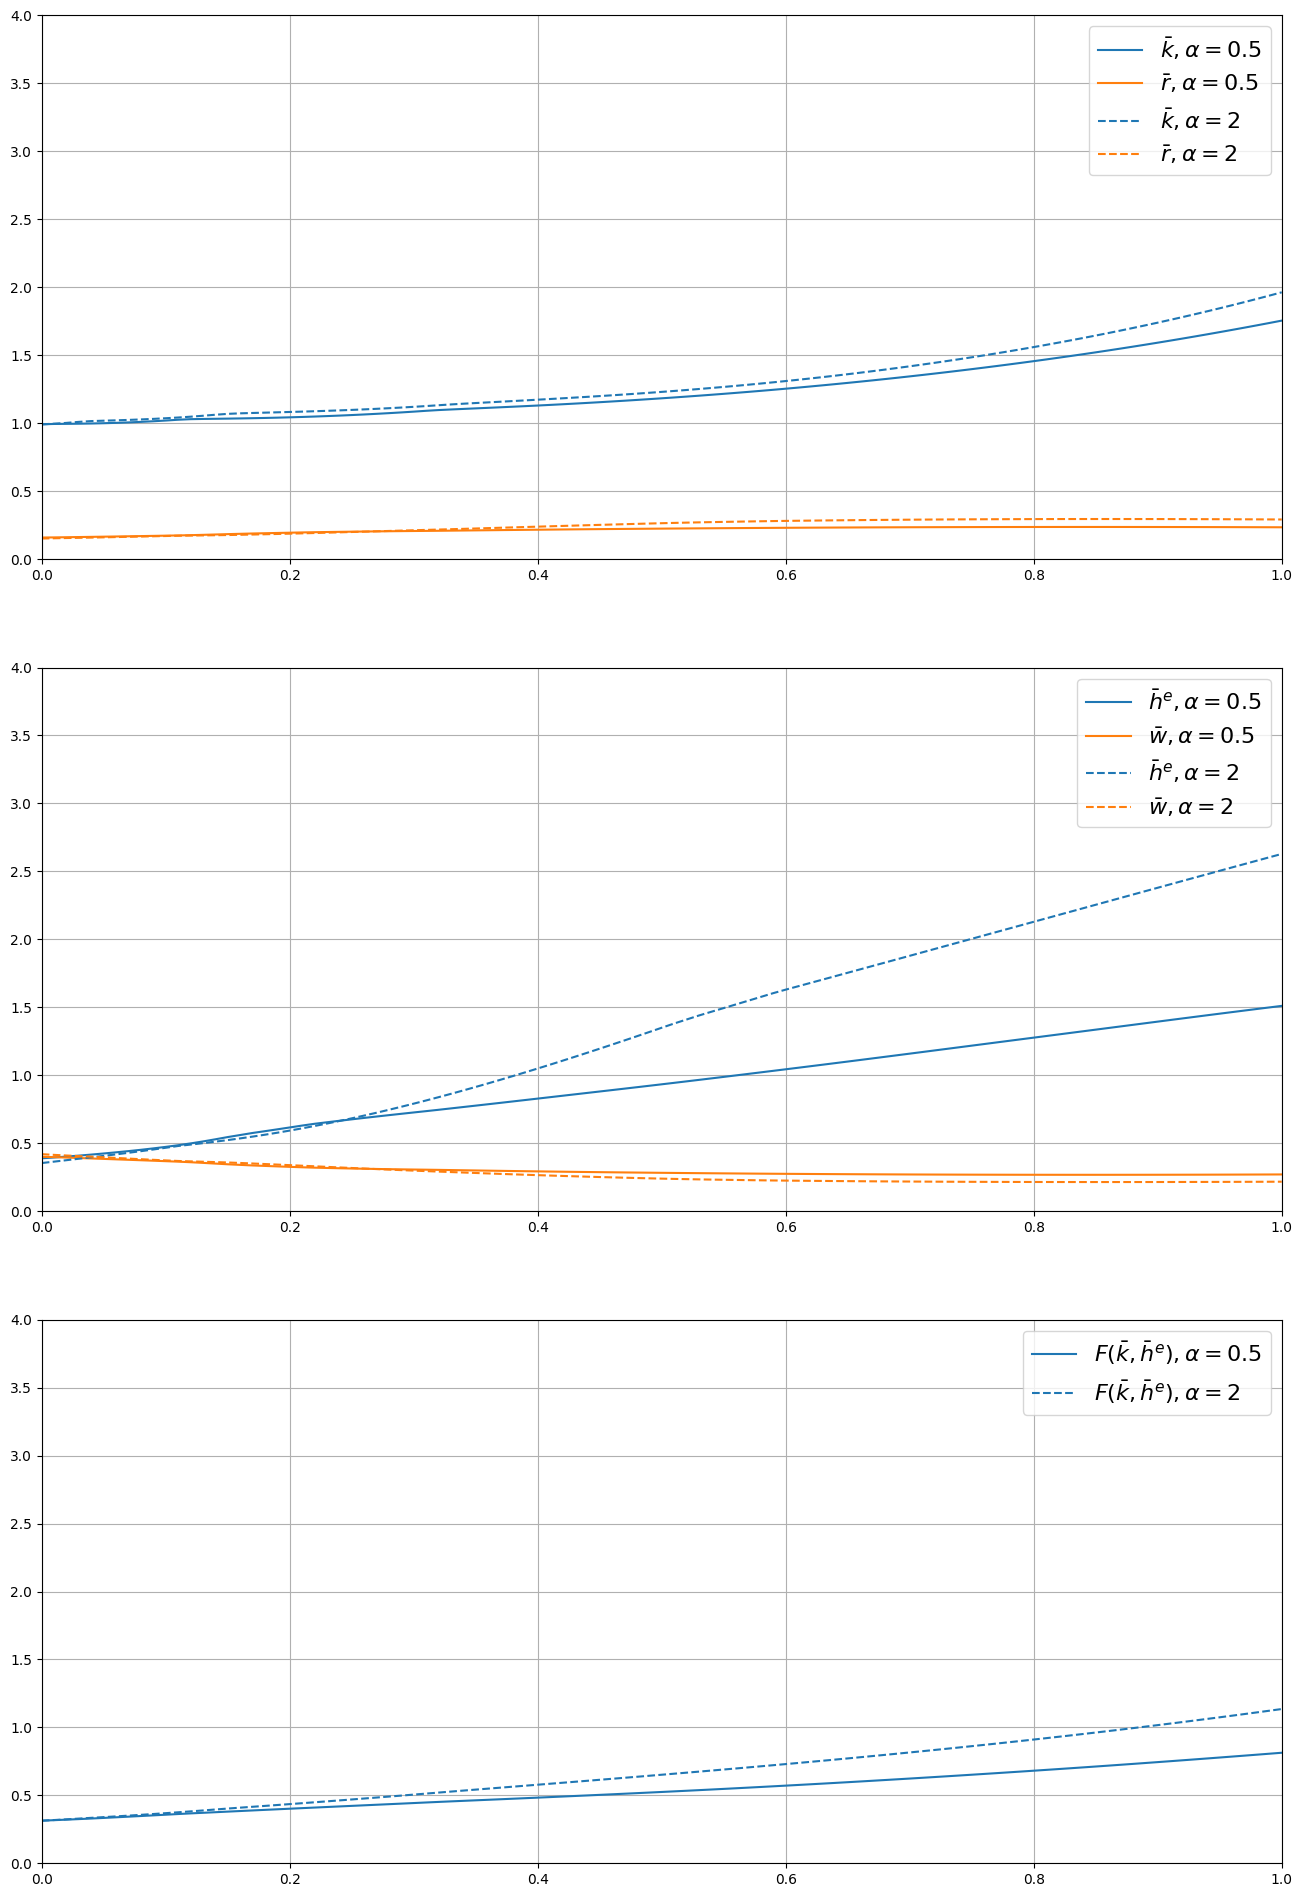
\includegraphics[width=\textwidth]{simulations_mfg.png}



\section{Conclusion}

\appendix
\addcontentsline{toc}{section}{Appendices}
\section*{Appendices}
\section{A little bit of game theory}\label{appendix-game-theory}
To Do
\begin{itemize}
    \item Games - definition - ok, 
    \item Strategies - ok, 
    \item Pure Strategies vs Mixed Strategies, - ok
    \item Nash Equilibrium, - ok 
    \item Stackelberg Equilibrium,  - ok
    \item Open Loop, - ok
    \item Closed Loop. - ok
    \item Seminal works in game theory
    \item Historical development
\end{itemize}

\subsubsection{Key Concepts}
\begin{enumerate}
    \item \textit{Game Theory} - area of mathematics concerned with the interaction of \textit{strategies} adopted by \textit{players} in order to maximize their \textit{payoff}. At the end of the day, a game is a system of optimization problems for which there is some interaction on the optimization target.
    \item \textit{Strategy} - an entity $x_i \in \mathcal{X}_i$ which represents one option, or control, that a player is allowed to choose, and which will be an input for the payoff function. Players want to choose their strategy in order to maximize their own payoff, while taking into account that the other players are doing the same thing.
    \item \textit{Pure vs Randomized (or mixed) Strategies}: A randomized strategy for player $i$ is a probability measure $\mu_i$ on the set of strategies $X_i$. A pure strategy is a randomized strategy with all of its mass concentrated on a single $x_i \in \mathcal{X}_i$%.  https://en.wikipedia.org/wiki/Strategy_(game_theory)#Mixed_strategy
    \item \textit{Player} - one player is equivalent to one dimension of the system of optimization problems.
    \item \textit{Payoff} - the optimization target of each player. The payoff for every player depends on the strategy chosen by every player. In the case of randomized strategies, the payoff is the expected value of the payoff function under the joint probability measure of the straties of all players.
    \item \textit{Solution concepts:} Nash Equilibrium, Stackelberg Equilibrium, Pareto Optimality.
        
        In general players cannot get the maximum payoff together. Different concepts of equilibrium are introduced in order to propose solutions to different kinds of games, which might differ by choice structure or cooperation possibility. Let`s consider the 2-dimensional case of two players, with sets of strategies denoted by $A,B$ and payoff functions $J_i: A\times B \mapsto \mathbb{R}$ for $i$ in $\{A,B\}$
    \begin{itemize}
        \item \textit{Pareto Optimality}: A pair of strategies $(a^*, b^*)$ is said to be \textbf{Pareto optimal} if there is no other pair $(a,b) \in A \times B$ such that
        $$
        J_A (a,b) > J_A(A^*, b^*) \text{ and } J_B(a,b) \geq J_B(a^*, b^*),
        $$
        or
        $$
        J_B(a,b) > J_B(a^*, b^*) \text{ and } J_A(a,b) \geq J_A(a^*,b^*).
        $$
        This means that is not possible to striclty increase the payoff of one player without strictly decreasing the payoff of the other.
        \item \textit{Nash Equilibrium}: A pair of strategies $(a^*,b^*)$ is said to be a \textbf{Nash Equilibrium} if $\forall a \in A, b\in B$, we have $J_A(a,b^*) \leq J_A(a^*,b^*)$ and $J_B(a^*,b) \leq J_B(a^*,b^*)$.
        This is a solution concept for a non-cooperative game. It is a situation in which no player can increase his payoff by changing his strategy if the other players do not change theirs. 
        \item \textit{Stackelberg Equilibrium}: Solution for a game with asymmetry of information. Let $R^B(a)$ be the set of best possible replies of Player $B$ if Player $A$ has announced the strategy $a$, that is, 
        $$R^B(a) = \{b' \in B : J_B(a,b) \leq J_B(a,b'), \forall b \in B\}.$$
        Then, a pair of strategies $(a^*,b^*) \in A\times B$ is a \textbf{Stackelberg Equilibrium} if 
        $$b^* \in R^B(a^*) \text{ and } J_A(a,b)\leq J_A(a^*, b^*),\ \forall(a,b), b\in R^B(a), a \in A.$$
    \end{itemize}
    
    \item \textit{completely cooperative and zero-sum}
    \item \textit{Information structure}: 

    % Define a differential game as setting for the strategies
    The information available for the players determine the possible strategies to be taken. This means that different game situations might arise for different information structures. Two particular information structures of notice are the \textbf{open loop} case and the \textbf{feedback case}. 
    \textbf{Open loop strategies} are strategies that depend only on time $t \in [0,T]$, which arise in situations where the state of the system cannot be known. Thus, the set $X_i$ of strategies available for the $i$-th player wiil consist of all measurable functions $t \mapsto u_i(t)$ from $[0,T]$ into $U_i$. \textbf{Feedback} (or \textbf{Markovian}) strategies arise when each player $i$ can observe the state of the system, but does not know the strategy of other players. In this case, the strategy for player $i$ can depend on both the time and the state, that is, the set of available strategies for player $i$ is the set of measurable functions $(t,x) \mapsto u_i(t,x)$ from $[0,T] \times \mathbb{R}^n$ into $U_i$ 
    \item \textit{Target and Game set}
\end{enumerate}

\section{Mathematical background}\label{appendix-mathematical-background}

\subsubsection{Deterministic optimal control problems}\label{deterministic_optimal_control}

Single agent whose state is denoted by $x_t \in \RR^d$, for $t_0 \leq t\leq T$, where $T > 0$ is arbitrarily fixed. The case $T< \infty$ is referred to as the finite horizon optimal control problem.

$$\dot x_t = f(v_t,x_t),$$

where $f: \RR^m \times \RR^d \mapsto \RR^d$ is a given function and $v_t \in \RR^m$ is a control. Let $\mathcal{W} \coloneqq \left\{ v : [t_0, T] \mapsto W, v \in X \right\}$, where $X$ is a suitable function space.

Agent's preferences are expressed through a utility functional $J(u_t, x_t; t)$. For $t \in [t_0,T)$ this functional is given by 

$$
J(u,x,t) = \int_t^T u(v_s, x_s) ds + \Psi(x_T),
$$
where $u : \RR^m\times \RR^d \mapsto \RR$ is the instantaneous utility (or running cost) and $\Psi : \RR^d \mapsto \RR$ is the terminal payoff.

In the case $T = \infty$, we introduce a discount rate $\beta > 0$ and consider
$$
J_\beta (u,x;t) = \int_t^\infty e^{-\beta (s - t) u(v_s, x_s)} ds 
$$

The focus of this section will be a variant of the last problem, namely:

$$
J_\alpha (u,x;t) = \int_t^\infty e^{-\alpha (s - t) u(v_s, x_s)} ds + e^{-\alpha (T -t)} \Psi(x_T) 
$$

The single agent seeks to maximize $J_\alpha$ over all possible controls.
We define the value function $v(x,t)$ as

$$
V(x,t) = \sup_{v\in \mathcal{W}} J_\alpha (v, x ; t).
$$
This function is the maximum possible payoff for the agent at state $x$ in time $t$.

Assumptions on $f$ (for the problem to be addressed rigorously):
$$f \in C(\RR^m \times \RR^d, \RR^d),\, |f(v, x_1) - f(v, x_2)| \leq C_\theta |x_1 - x_2|, x_1, x_2 \in \RR^d, v\in \RR^m, |v| \leq \theta$$

If the Value function is of class $C^1(\RR^d \times [t_0,T])$, it solves  a nonlinear partial differential equation known as the Hamilton-Jacobi equation:
$$V_t(x,t) - \alpha V(x,t) + H(x,D_x V(x,t)) = 0,$$
where the Hamiltonian H is defined as 
$$H(x,p) = \sup_{v\in W} [p \cdot f(v,x) + u(v,x)],$$
that is, the Legendre transform of the running cost $u$.
The optimal control $v_t^*$ is given by 
$$ H_p (x^*, D_x V(x^*,t)) = f(v^*, x^*)$$


\begin{proposition}[Dynamic programming principle]
    Let $r \in (t_0, T)$ be fixed and assume that $V$ is a value function. Then we have
    $$
    V(x,t) = \sup_{v\in \mathcal{W}} \left( \int_r^T e^{-\alpha (s-r)} u(v_s,x_s) ds + e^{-\alpha (r - t) V(x_r,r)} \right).
    $$
\end{proposition}

\begin{proof}
    To do
\end{proof}

\begin{proposition}[Verification Theorem]
    Let $U \in C^1(\RR^d \times [t_0, T])$ be a solution to 
    $$
    U_t(x,t) - \alpha U(x,t) + H(x, U_x(x,t)) = 0\, \text{(HJ)}
    $$
    where 
    $$
    H(x,p) = \sup_{v \in W} [p \cdot f(v,x) + u(v,x)],
    $$
    with terminal condition $U(x,T) = \psi(x)$. Then
    $$U(x,t) \geq V(x,t), \forall (x,t) \in \RR^d \times [t_0,T].$$
    Moreover, if there exists a control $v^*$ such that
    $$
    H(x^*_t, U_x (x^*_t, t)) = U_x(x^*_t, t)\cdot f(v^*_t, x^*_t) + u(v^*_t, x^*_t),
    $$
    That is, $v^*$ gives an equality in the Hamiltonian, then $v^*$ is an optimal control for the control system and $U(x,t) = V(x,t)$.
\end{proposition}

\begin{proof}
    To do
\end{proof}


\subsubsection{Transport Equation}\label{transport_eq}
Consider a population that is governed at the single agent level by
\begin{equation}\label{transport_eq:ode}
\begin{cases}
    \dot x_t = b(x_t,t), \quad t > t_0,\\
    x_{t_0} = x.
\end{cases}
\end{equation}
where $b$ is a Lipschitz vector field. The vector field induces a flow that trasports the population's density along time (pushforward). The evolution of the density is described be the \textit{transport equation}, a first order pde:  

\begin{equation}\label{transport_eq:pde}
\rho_t + \Delta(b(x,t) \rho) = 0.
\end{equation}

\begin{proposition}[Properties of solutions]    
Let $\rho$ be a solution of \eqref{transport_eq:pde} with initial condition $\rho(x,t_0) = \rho_0(x)$, for some probability density $\rho_0 \in \mathcal{C}_c^\infty (\RR^d).$ Then we have:
\begin{itemize}
    \item Positivity of solutions: $\rho(x,t) \geq 0$ for all $t> t_0$,
    \item Mass conservation: $\int_{\RR^d} \rho(x,t) dx = \int_{\RR^d} \rho_0(x) dx = 1$ for all $t > 0$.
\end{itemize}
\end{proposition}

\begin{proof}
    To do.
\end{proof}

Define the flow in $\RR^d$ given by $b$ by $\Phi_t$. This flow maps $x\in \RR^d$ to the solution of \eqref{transport_eq:ode} at the instant $t > t_0$, with initial condition $x$.

We can use the operator $\Phi_t$ to define a family of measures $\theta(x,t)$ over $\RR^d$ from an initial measure $\theta_0$ by 
\begin{equation}\label{transport_eq:family_of_measures}
\int_{\RR^d} \phi(x) \theta(x,t) dx = \int_{\RR^d} \phi(\Phi_t(x)) \theta_0 dx    
\end{equation}

This measure satisfies the transport PDE in the distribution sense. 
\begin{proposition}[Solutions in the distribution sense]
Let $\theta$ be the measure defined in \eqref{transport_eq:family_of_measures}. Assume that the vector field $b$ is Lipschitz continuous and denote by $\Phi_t$ the flow corresponding to \eqref{transport_eq:ode}. Then
\begin{equation}\label{transport_eq:pde_for_measures}
    \begin{cases}
        \theta_t(x,t) + \Delta(b(x,t) \theta(x,t)) = 0, \quad (x,t) \in \RR^d \times [t_0,\infty),\\
        \theta(x,t_0) = \theta_0(x), \quad x\in \RR^d.
    \end{cases}
\end{equation}
in the distributional sense.
\end{proposition}

\begin{proof}
    To do.
\end{proof}

\begin{proposition}[Dirac delta solution]\label{transport_eq:prop:dirac_delta_solution}
Assume that \eqref{transport_eq:ode} holds and suppose that $b$ is Lipschitz continuous. Then, $\delta_{\Phi_t(x)}$ solves \eqref{transport_eq:pde_for_measures} in the distributional sense.
\end{proposition}

\begin{proof}
    To do.
\end{proof}

\begin{remark} The converse of \eqref{transport_eq:prop:dirac_delta_solution} also holds.
\end{remark}

\printbibliography

\end{document}